\section{数据库设计}
\subsection{系统数据流设计}
热点发现和舆情分析中数据是重中之重。网络数据具有信息量大、更新速度块的特点,且网络热点话题具有一定的时效性,因此需要从数据获取到结果展示,要有及时、稳定和高效的流程。系统的核心数据流主要为数据获取到数据存储数据流和数据存储到前端展示数据流。
本系统使用多种形式的数据源。与市面常见的舆情监控系统相比较,一大优势在于数据源多。传统的舆情监控系统多数只采用媒体新闻数据或单一的新浪微博数据。本系统不仅包含媒体新闻数据、主流门户(sohu、网易、新浪)评论数据、新浪微博数据还使用公司内部的说说、兴趣部落数据和电脑管家、浏览器搜索日志,将社交数据和搜索日志也加到热点舆情发现与分析中。综上,恰当的数据流设计,至关重要。

\subsubsection{数据获取到数据存储数据流设计}
网络数据的获取来源主要包含外网下载和内部推送。
外网下载的数据包括媒体新闻数据、主流门户(sohu、网易、新浪)评论数据和新浪微博数据。外网下载依托spider下载平台,对网页数据进行抓取,并通过通用抽取和特定抽取流程获得结构化信息。Spider下载平台的能够通过下载机器的扩容,提升下载量,每日千万级网页的下载,能够满足本系统的需求。对于普通站点新闻的下载结果使用通用抽取即可满足需求,但对于评论数据和新浪微博数据需要定制特定的抽取程序。
内部推送即使用公司内部数据,直接按照指定格式进行推送。内部推送数据包括快报新闻数据、tx新闻评论数据、说说兴趣部落数据和电脑管家、浏览器搜索日志。内部推送的快报新闻数据和tx新闻评论数据,避免了下载、抽取步骤对数据处理的实时性和准确性有了大大的提升。电脑管家、浏览器搜索日志是生成搜索指数的重要来源。说说、兴趣部落数据是生成社交指数的重要来源。
数据获取后对新闻数据进行新闻预处理,将处理后的数据一份推送到Hadoop进行存储备份和热点发现使用,另一份推送按指定字段建立索引,并存储到检索系统中,方便之后流程的使用。同样,对新闻评论数据进行评论预处理,按指定字段建立索引存储到检索系统。除此之外,直接对新浪微博数据, 兴趣部落数据和搜索日志数据,建立索引,存储到检索系统中。

\subsubsection{数据存储到前端展示数据流设计}
从Hadoop集群中取得最新的一个小时内的媒体数据,对标题进行热点聚合,得到热点话题和相应关键字列表。在检索系统中按关键字对媒体新闻数据进行检索,并对检索结果进行计算得到词云、媒体渠道分布、媒体热度趋势数据。对社交数据进行检索计算得到社交渠道分布、社交热度趋势和社交情感趋势数据。对评论数据进行检索计算得到媒体情感分布和用户代表观点。
得到上述数据,存入Mysql数据库中,方便前端展示。
最后,前端通过对Mysql数据库中数据的使用,展示数据并实现业务逻辑。

\subsection{系统数据库设计}
热点发现与线索管理系统和舆情系统,数据和业务之间存在一定的耦合。热点发现与线索管理系统主要为个人提过内容生产服务,也会对热点的相关舆情进行分析。舆情系统是对企业提供舆情服务,对企业制定舆情服务,进行舆情监控与报警。针对这些耦合,两个系统后台使用同一数据库,按不同的业务逻辑进行定制和展示。
数据库中数据表较多,选取具有代表性的表进行展示。
版本控制表是整个数据库中的核心表,通过versionid在不删除和覆盖其他相关表中数据的情况下进行相关数据的更新。版本控制表如下表所示,以versionid为主键,按 versionid或topicid根据不同的需要与其他表做关联。

% Please add the following required packages to your document preamble:
% \usepackage{longtable}
% Note: It may be necessary to compile the document several times to get a multi-page table to line up properly
\begin{longtable}[c]{|l|l|l|l|l|}
	\caption{版本控制表}
	\label{tab:my-table}\\
	\hline
	字段          & 数据类型         & 主键 & 是否可控 & 备注   \\ \hline
	\endfirsthead
	%
	\multicolumn{5}{c}%
	{{\bfseries Table \thetable\ continued from previous page}} \\
	\endhead
	%
	versionid   & int(11)      & 是  & 否    & id自增 \\ \hline
	date        & varchar(32)  & 否  & 否    & 数据日期 \\ \hline
	topicid     & varchar(100) & 否  & 否    & 热点id \\ \hline
	keyscontent & varchar(128) & 否  & 否    & 关键词  \\ \hline
	trade       & varchar(40)  & 否  & 否    & 一级行业 \\ \hline
	strade      & varchar(40)  & 否  & 否    & 二级行业 \\ \hline
	addtime     & timestamp    & 否  & 否    & 添加日期 \\ \hline
\end{longtable}

热门话题日数据表如下表所示。与热门话题日数据表结构相类似的还有热门话题周数据表、热门话题月数据表、突发事件数据表、头条新闻数据表和搜索排行数据表等。

% Please add the following required packages to your document preamble:
% \usepackage{longtable}
% Note: It may be necessary to compile the document several times to get a multi-page table to line up properly
\begin{longtable}[c]{|l|l|l|l|l|}
		\caption{热门话题数据表}
	\label{tab:my-table1}\\
	\hline
	字段               & 数据类型         & 主键 & 是否可控 & 备注         \\ \hline
	\endfirsthead
	%
	\multicolumn{5}{c}%
	{{\bfseries Table \thetable\ continued from previous page}} \\
	\endhead
	%
	id               & int(11)      & 是  & 否    & id自增       \\ \hline
	category         & varchar(50)  & 否  & 否    & 一级类别       \\ \hline
	category2        & varchar(200) & 否  & 否    & 二级类别       \\ \hline
	classes          & varchar(50)  & 否  & 否    & 渠道         \\ \hline
	topicid          & varchar(64)  & 否  & 否    & 标题         \\ \hline
	name             & varchar(50)  & 否  & 否    & 热度         \\ \hline
	info             & varchar(120) & 否  & 否    & URL链接      \\ \hline
	impact           & int(11)      & 否  & 否    & 相关文章个数     \\ \hline
	timestamp        & int(11)      & 否  & 否    & 热点开始时间     \\ \hline
	reputation       & varchar(100) & 否  & 否    & 热点评论数      \\ \hline
	heat             & int(11)      & 否  & 否    & 热度         \\ \hline
	locationlist     & varchar(64)  & 否  & 否    & 地点列表       \\ \hline
	versionid        & int(8)       & 否  & 否    & 版本数据       \\ \hline
	detailflag       & tinyint(1)   & 否  & 否    & 标识符(有无详情页) \\ \hline
	mediahot         & int(1)       & 否  & 否    & 媒体热度       \\ \hline
	socailhot        & int(11)      & 否  & 否    & 社交热度       \\ \hline
	searchhot        & int(11)      & 否  & 否    & 搜索热度       \\ \hline
	imageurl         & varchar(256) & 否  & 否    & 图片地址       \\ \hline
	personlist       & varchar(256) & 否  & 否    & 人物列表       \\ \hline
	organizationlist & varchar(256) & 否  & 否    & 机构单位       \\ \hline
	cloudwordlist    & text         & 否  & 否    & 词云         \\ \hline
	keywordlist      & varchar(256) & 否  & 否    & 关键词列表      \\ \hline
	addtime          & datetime     & 否  & 否    & 入库时间       \\ \hline
\end{longtable}

用户企业与告警对象一对多联系。一个用户企业可以设置多个告警对象, 监测不同方面舆情,但一个告警对象只能属于特定的用户企业。告警对象与告警配置一对多联系。一个告警对象可以设置多个告警配置,但一个告警配置只能归属于一个告警对象。告警对象与告警内容一对多联系。一个告警对象可以有多条告警内容,但一个告警内容只能归属于一个告警对象。告警文章与告警内容多对多联系。一篇告警文章可以对应多个告警内容,一个告警内容也可以对应多篇告警文章。舆情告警相关数据库设计图如下图所示。

\begin{figure}[!htbp]
	\centering
	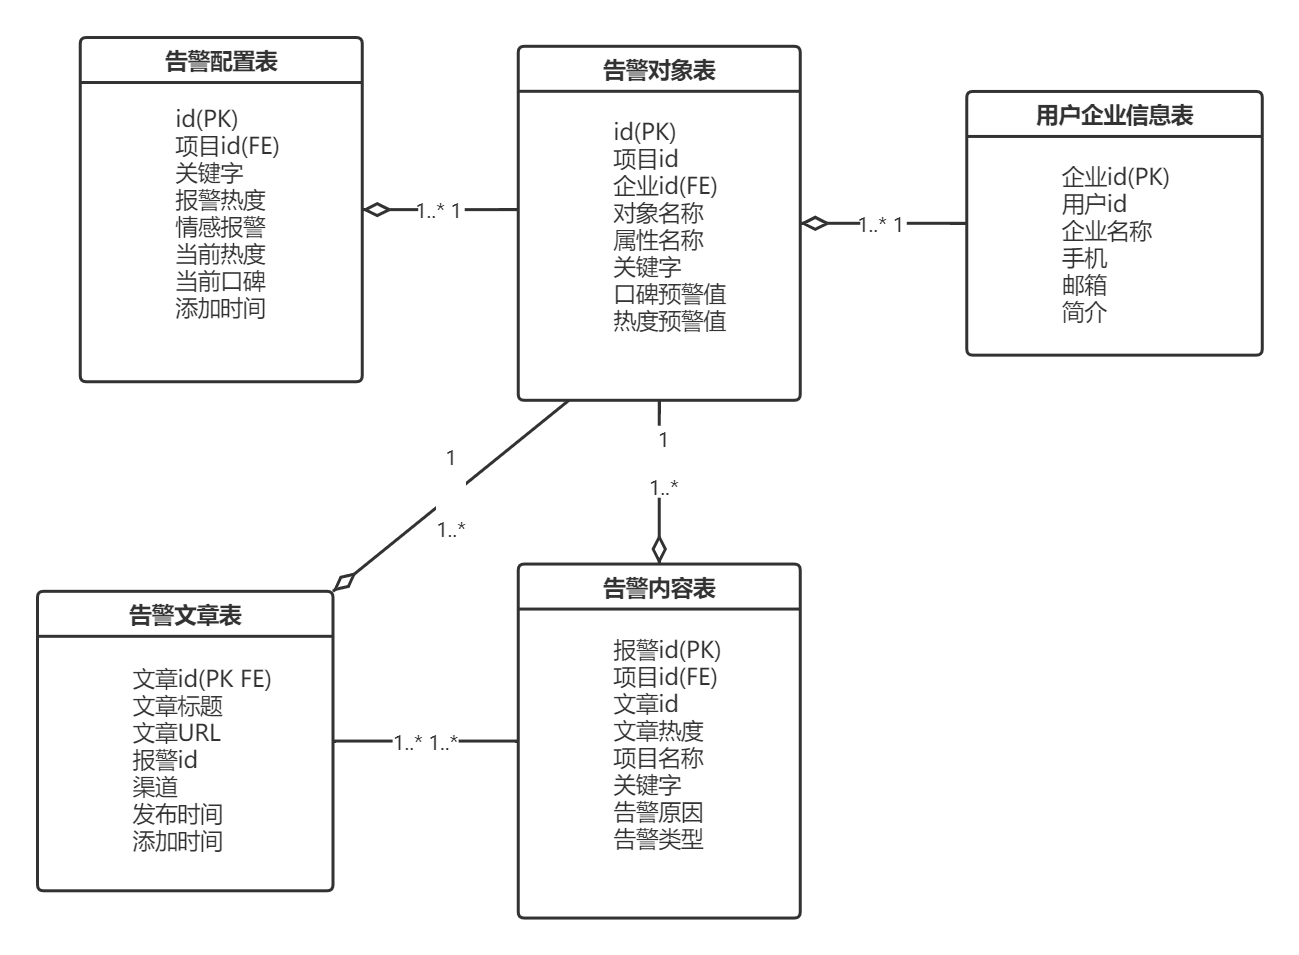
\includegraphics[scale=0.3]{image/d1.png}
	\caption{舆情告警数据库设计图}
\end{figure}

舆情分析数据库设计图如下

\begin{figure}[!htbp]
	\centering
	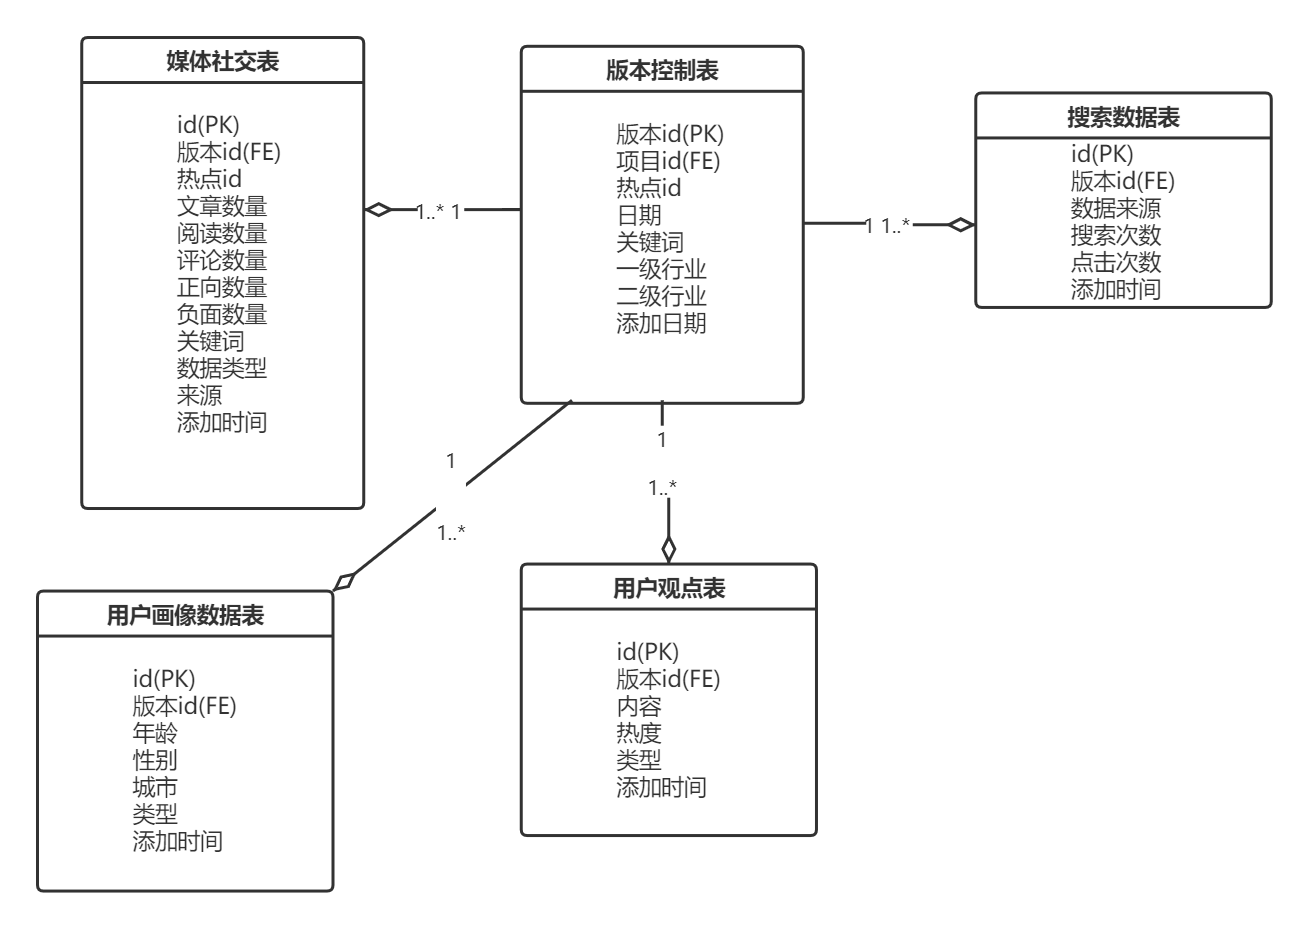
\includegraphics[scale=0.3]{image/d2.png}
	\caption{舆情分析数据库设计图}
\end{figure}
